%
%%%%%%%%%%%%%%%%%%%%%%%%%%%%%%%%%%%%%%%%%%%%%%%%%%%
%
%  E N T W I C K L U N G S U M G E B U N G
%
%%%%%%%%%%%%%%%%%%%%%%%%%%%%%%%%%%%%%%%%%%%%%%%%%%%
\chapter{Grundlagen}
\label{cha:grundlagen}
%
%
In dem Grundlagenkapitel geht es um das Basiswissen, auf dem die Arbeit aufbaut. Es wird näher auf die verwendeten Technologien eingegangen. Dabei werden die Frontend-Frameworks beleuchtet sowie die 3D Bibliotheken. Näher wir auch auf die Begriffe Resposive Webdesign, Usability und Performance eingegangen.
%
%
%%%%%%%%%%%%%%%%%%%%%%%%%%%%%%%%%%%%%%%%%%%%%%%%%%%
%
% S P A
%
%%%%%%%%%%%%%%%%%%%%%%%%%%%%%%%%%%%%%%%%%%%%%%%%%%%
%
\section{Single Page Anwendungen}
\label{sec:spa}
%
Früher war es bei Webanwendungen wichtig, soviel wie möglich auf dem Server zu erledigen. Bei modernen Webframeworks gilt jedoch genau das Gegenteil. Es wird versucht möglichst viel clientseitig umzusetzten.\textit{\glqq Dies steigert die Benutzerfreundlichkeit und schafft die Möglichkeit der Anpassung an die Auflösungen und Formfaktoren der vielen unterschiedlichen klassischen und mobilen Plattformen.\grqq } \cite{bahor_html5/webgl_2013}. Im Folgenden wird nun kurz etwas genauer darauf eingegangen was André Krämer in seinem Videokurs sehr gut und einfach erklärt hat.
%
\paragraph{Klassische Webanwendungen}
%
Bevor man sich damit befasst was Single Page Anwendungen sind, sollte man sich das Prinzip einer klassischen Webanwendung anschauen. Nehmen wir beispielsweise an, ein Client sendet eine Anfrage an einen Server. Hierbei handelt es sich um einen Webbrowser, welcher eine Webadresse öffnen möchte. Der Zielserver übernimmt die Verarbeitung. In der Regel laufen nun Skripte auf dem Server, welche HTML rendern. Schließlich bekommt der Client auf seine Anfrage eine Antwort in Form eines HTML-Dokumentes und kann es dann anzeigen. Bei diesem Vorgang liegt die komplette Verarbeitung bei dem Server. Der Webbrowser dient lediglich der Darstellung und einfachen Eingabe. Das die Daten auf einem Server verarbeitet werden wird deutlich, wenn ein Seitenwechsel vorgenommen wird. Dabei wird kurze Zeit nichts angezeigt während die Seite komplett neu lädt.\\
Mit der Einführung von AJAX\footnote{Ajax bzw. AJAX steht als Akronym für „Asynchronous JavaScript and XML“. Die Technologie ermöglicht es, einzelne Teile einer Webseite bei Bedarf asynchron zu laden, so dass sie dynamisch wird. Der angezeigte Inhalt lässt sich gezielt so manipulieren, ohne die komplette Seite neu zu laden.} in 2005 machte die Webentwicklung einen Schritt nach vorne. Nun war es nämlich möglich, Daten asynchron an den Server zu senden. Das heißt, der Server verabreitet zwar immer noch die Daten, sendet nun aber nur noch einen Teil des vorgerenderten Dokuments oder sogar nur einzelne Daten der Seite. Somit wird die Seite nicht wieder komplett neu geladen. Wenn man nun aber in einen komplett andern Bereich der Seite wechseln will, hilft AJAX nicht. Die Seite wird neu geladen und es dauert einen kurzen Moment bis das Ergebnis vom Webbrowser angezeigt werden kann. Um dieses Problem zu lösen, kommen \textit{Single Page Anwendungen} zum Einsatz.
\paragraph{Dezentralisierung der Webanwendung}
%
Im Grunde arbeiten SPA's nach folgendem Prinzip: Der Webbrowser sendet eine Anfrage an den Server. Dieser verarbeitet, wie bei klassischen Webanwendungen nun die Anfrage. Anschließend wird im Webbrowser eine Benutzeroberfläche dargestellt. Nun kommt der entscheidende Unterschied zu klassischen Anwendungen. Bei einem Seitenwechsel oder anderen Interaktionen des Benutzers wird eine neue Benutzeroberfläche erzeugt, indem Teile der Seite ausgetauscht werden. Die Seite wird nie komplett neu geladen. Der Nutzer bleibt immer auf der einen Seite, zumindest fühlt es sich für den Benutzer so an. Dieses Prinzip kennt der Anwender von Desktop-Anwendungen. Man hat sogar die Möglichkeit die Anwendung (zumindest teilweise) offlinefähig zu machen.\\
Die Grundlage einer solchen Anwendung ist das Routing. Abhängig vom Pfad werden bestimmte Bausteine der Anwendung angezeigt bzw. ausgeblendet. Wie wir im späteren Verlauf dieser Arbeit noch sehen werden, hat man tatsächlich nur eine HTML-Datei, welche abhängig vom Kontext immer andere Inhalte anzeigen kann.\\
%
Zusammenfassend lässt sich also festhalten, das ein Ziel von SPAs ist, die Kommunikation zwischen Client und Server enorm zu reduzieren. Um dies zu erreichen wird die Anwendung dezentralisiert. Das heißt, es gibt nur ein HTML Dokument\cite{domin_was_2018}. Durch den Einsatz von Frameworks, wie Angular, ist es möglich Inhalte zu aktualisieren oder zu einer anderen Seite zu wechseln, ohne die Seite über den Server neu zu laden.
\footnote{Das Prinzip von Single Page Anwendungen wird zum Beispiel von Googles Gmail und Gmaps sowie von Twitter verwendet}
%
%
%%%%%%%%%%%%%%%%%%%%%%%%%%%%%%%%%%%%%%%%%%%%%%%%%%%
%
% A U F B A U 
%
%%%%%%%%%%%%%%%%%%%%%%%%%%%%%%%%%%%%%%%%%%%%%%%%%%%
%
\section{Framework Angular}
\label{sec:angular7}
Das Framework Angular ist sehr umfangreich. Im Folgenden werden einige Grundlagen erläutert, die zur Implementierung einer Anwendung mit Angular benötigt werden. Dabei soll ein Grundverständis vermittelt werden, wie das Framework aufgebaut ist und wie es arbeitet.
\subsection{Komponentenbasierte Programmierung}
%
Angular ist ein Framework, das auf Komponenten setzt. Das Prinzip der komponentenbasierten Entwicklung kommt nicht nur bei Angular vor, sondern auch bei vielen anderen Programmiersprachen und Frameworks. Was in Angular Komponenten sind wird in dem Buch \textit{Angular: Grundlagen, fortgeschrittene Techniken und Best Practices mit TypeScript - ab Angular 4, inklusive NativeScript und Redux} folgendermaßen beschrieben:\\
%

\textit{\glqq Komponenten sind die Grundbausteine einer Angular Anwendung. Jede Anwendung ist aus vielen verschiedenen Komponenten zusammengesetzt, die jeweils eine bestimmte Aufgabe erfüllen. Eine Komponente beschreibt somit immer einen kleinen Teil der Anwendung, z. B. eine Seite oder ein einzelnes UI-Element.\grqq }\cite{woiwode_angular:_2017} \\

%
Im Grunde ist eine Komponente also nichts anderes als ein selbstdefinierter HTML-Knoten, den man im HTML Kontext ganz normal nutzen kann. Man erzeugt einfach DOM-Elemente\footnote{Wenn eine Webseite geladen wird, erstellt der Browser eine Document Object Model der Seite. Das HTML-DOM-Modell ist als Baum von Objekten aufgebaut. Diese Objekte sind ein der Regel einfache HTML-Tags} und kann sie dann automatisch in Angular nutzen.
Eine Komponente in Angular ist in drei Parts aufgeteilt: Logik, Vorlage und Style. Die Logik beschreibt die TypeScript Klassen, Eigenschaften, Methoden und so weiter. Sie beschreibt also, was zu tun ist, wenn zum Beispiel ein bestimmter Button geklickt wird. Die Vorlage (Template) ist ein HTML-Schnipsel. Dies kann einfach nur ein Button-Element sein oder auch eine HTML-Struktur mit mehreren HTML-Elementen. Sie beschreibt die Stuktur bzw. den Aufbau der Komponente. Wie die Komponente aussehen soll wird in dem Style Part festgelegt. Dabei ist zu beachten, dass die Style-Definitionen nur innerhalb der Komponente gelten. Globale Styles der Anwendung werden seperat definiert.\\
Der Startpunkt der Anwendung ist die \texttt{index.html}. Sie definiert die Applikationskomponente, der Ankerpunkt einer Angular-Anwendung, quasi eine Basiskomponente. In Dieser können nun weitere Kindskomponenten eingefügt werden, welche auch ineinander verschachtelt sein können. So entsteht eine komplette Struktur. Eine Komponentenvorlage kann also nicht nur HTML-Elemente enthalten, sondern auch Kindskomponenten. Entscheidend ist, das Komponenten verschachtelt werden können. Dies ist das Grundprinzip der komponentenbasierten Programmierung (vgl. Angular Grundkurs\cite{unlu_angular_2018}).

\subsection{Modulare Umsetzung}
Schauen wir uns nun an, wie Angular mit Modulen arbeitet und was genau Module sind. \textit{Nikolas Poniros} hat das in seinem Buch \textit{Angular für Dummies} so definiert:\\

\textit{\glqq Angular-Module helfen beim Gliedern einer Webanwendung in verschiednene Funktionsblöcke. Alle Angular-Bausteine, die logisch zu einem Funktionsblock gehören, werden mit dem entsprechenden Angular-Modul registriert. Die registrierten Bausteine gehören dann zum Angular-Modul. Angular-Module sind von der Denkweise her vergleichbar mit ECMA-Script-Modulen. ECMA-Script-Module kapseln TypeScript-Konstrukte wie Klassen und Funktionen und erlauben nur den Zugriff auf exportierte Konstrukte. Angular-Module kapseln Komponenten, Pipes und Direktiven\footnote{Was genau es mit diesen Angular Bausteinen auf sich hat wird in Punkt \ref{subsec:grundfunktionen} beleuchtet.}. Ein anderes Angular-Modul kann nur auf einen Baustein zugreifen. wenn es dieses exportiert.\grqq \cite{poniros_angular_2019} }\\

Angular bietet also die Möglichkeit modular zu arbeiten. Die einzelnen Elemente und Funktionalitäten können in Modulen gruppiert werden. Im Grunde ist ein Modul nichts anderes als ein Container. Sie lassen sich besonders gut verwenden, wenn man mit mehreren Entwicklern zusammenarbeiten möchte. Module sind einzelne Bestandteile der Anwendung und lassen sich ganz einfach in bestehende Anwendungen einbauen. So kann ich ein Modul in mehreren Anwendungen wiederverwenden. Oder verschiedene Teammitglieder entwickeln jeweils ihre eigenen Module, welche anschließend in einer Anwendung zusammengefügt werden können. Ich kann ein Modul also auch in einem anderen Kontext wiederverwenden. Ein Modul darf allerdings nur in einem einzigen Modul initialisiert werden. Stattdessen wird das Modul bei mehrfacher Verwendung lediglich importiert. Folgendes Beispiel soll das Prinzip modularer Umsetzung verdeutlichen.\\
%
\begin{figure}[h]
	\centering
	{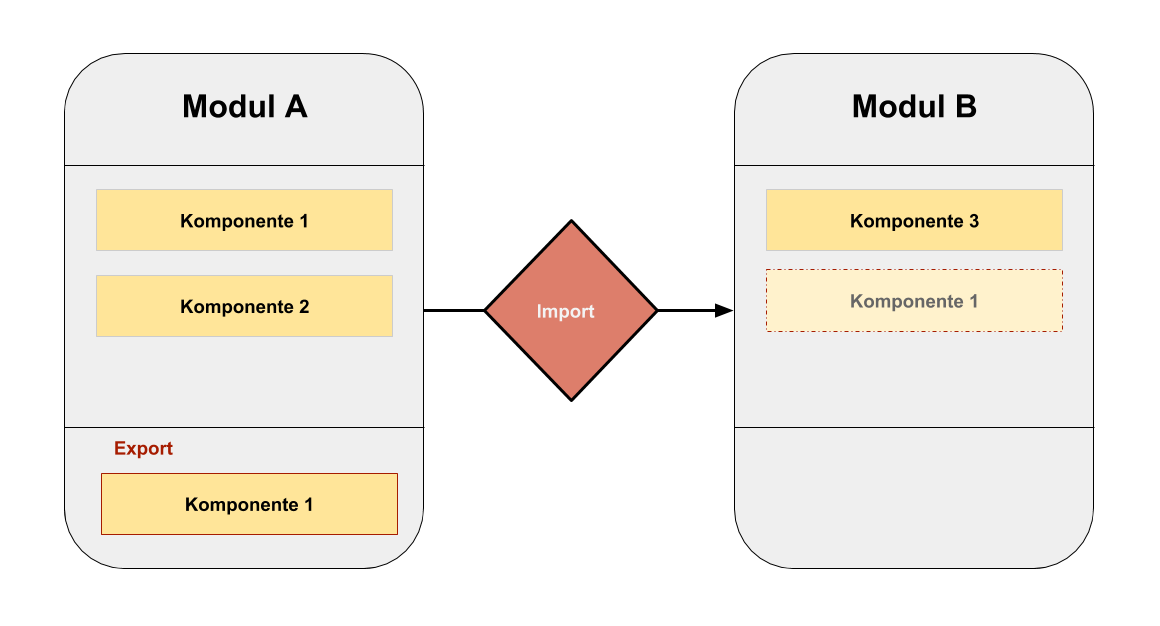
\epsfig{file = grundlagen/images/module.png, width=14.0cm}}
	\caption[Angular Modul Beispiel]{\textit{Fallbeispiel mit zwei Angular Modulen mit Komponenten}}
	\label{fig:ngModule}
\end{figure} 
%
Das hier beschriebene Beispiel ist in Abbildung \ref{fig:ngModule} zu sehen. Angenommen wir haben ein \textit{Modul A}. In diesem Modul sind nun \textit{Komponente 1} und \textit{Komponente 2} deklariert. Das heißt, es ist möglich in \textit{Komponente 1} die \textit{Kompontente 2} zu verwenden und umgekehrt, weil beide in dem \textit{Modul A} registriert sind. Jetzt haben wir ein weiteres \textit{Modul B}. In diesem ist die \textit{Komponente 3} registriert. Nun wäre es sehr praktisch, wenn \textit{Komponente 3} ebenfalls \textit{Komponente 1} aus dem anderen Modul verwenden könnte. Wie schon erwähnt darf ein Baustein in Angular nur in einem Modul registriert bzw. inititalisiert werden. Deshalb muss das \textit{Modul A} in \textit{Modul B} importiert werden, damit auch dort die \textit{Komponente 1} verwendet werden kann. Zusätzlich muss in \textit{Modul A} die \textit{Komponente 1} exportiert werden. Dadurch wird sie erst von außen frei zugänglich und somit in Bausteinen anderer Module nutzbar.
%
\paragraph{Hauseigene Module}
Angular hat auch ein paar hauseigene Module, die je nach Anwendungsfall importiert werden können. Das \textit{BrowserModule} wird für Web-Anwendungen im Angular-Umfeld genutzt und verfügt über alle Funktionalitäten, mit dem wir in der Lage sind, Ereignisse innerhalb des Browsers abzufangen, DOM-Rendering durchführen zu können und damit schließlich die lauffähige Angular-Anwendung im Browser realisieren zu können.\\
Das \textit{CommonModule} beinhaltet allgemeine Funktionen, die sehr, sehr häufig genutzt werden. Diese Funktionen liegen in Form von Direktiven und Pipes vor, womit ich bestimmen kann, ob ein HTML-Knoten angezeigt wird oder nicht oder auch Pipes, womit ich Ausgaben formatieren kann. Auch sprachabhängige Funktionalitäten sind in den \textit{CommonModule} enhalten.\\
Das \textit{HttpModule} ist dafür da, Client-Server-Kommunikation zu betreiben. Das heißt, HTTP-Requests lassen sich mit Hilfe des \textit{HttpModules} hervorragend realisieren, dafür werden Services zur Verfügung gestellt. Das \textit{HttpModule} hat auch Services für Testings und Co. Für Formulare gibt es entweder das FormsModule oder das \textit{ReactiveFormsModule}. Das hängt so ein wenig davon ab, wie man Formulare in der Anwendung gestalten will.\\
Das \textit{RouterModule} ist dafür da, um Komponenten-Routing zu realisieren. Das Routing ist die Grundlage für \textit{Single-Page-Applications}. Das heißt, über das Routing kann man bestimmen, welche Komponente dargestellt werden muss, wenn ein bestimmter Pfad in der Anwendung besucht wird.
%
\subsection{Grundfunktionen des Frameworks}
\label{subsec:grundfunktionen}
%
Module und Komponenten in Angular haben wir nun schon etwas ausführlicher betrachtet. Nun wollen wir uns weitere Funktionen und Bestandteile von Angular anschauen\footnote{Auf die weiteren Bestandteile von Angular wird hier nicht im Details eingegangen. Genauere Dokumentationen dazu sind online unter angular.io zu finden.}. Wie die einzelnen Bausteine umgesetzt und implementiert werden können sehen wir noch in Kapitel 4 Methodik am Fallbeispiel des 3D Konfigurators für Mehrwegbecher.
%
\paragraph{Bindungen}
%
\textit{\glqq Bindungen sind im Wesentlichen die Brücke zwischen der Darstellungsschicht und der Logikschicht\grqq } \cite{unlu_angular_2018}. Man kann beispielsweise Variablen oder Eigenschaften aus TypeScript-Klassen in  Vorlagen binden. Angenommen in der TypeScript-Klasse einer Komponente ist die Variable \texttt{title} deklariert. Um \texttt{title} nun in der Vorlage zu binden, schreibt man Folgendes: \texttt{ <h1> \{\{title\}\} </h1>}. Natürlich geht das ganze noch deutlich komplexer. Dadurch wird die Komponente mit ihrem Content dynamisch.
%
\paragraph{Direktiven}
%
Direktiven sind ein wichtiger Bestandteil von Angular. Direktiven werden in Vorlagen genutzt, indem ich sie als Attribute auszeichne. Das heißt, Direktiven sind oft Attribute, die in ein HTML-Element hinzugefügt werden oder auch beispielsweise dadurch deklariert, dass an ein bestimmtes HTML-Element ein bestimmtes Attribut angehängt sein muss. Attribut-Direktiven machen eigentlich nichts anderes als eine Anpassung des Aussehens beziehungsweise eine Anpassung des Verhaltens eines Elements, das heißt, es manipuliert ein vorhandenes Element im Wesentlichen.\\
Analog dazu kann man auch strukturelle Direktiven benutzen. Das gibt es zum Beispiel \texttt{ngFor}, diese ist sehr praktisch bei der Entwicklung einer Angular-Anwendung. Sie benutzt nämlich das Element, auf das sie angewendet wurde, als Vorlage, iteriert durch eine Liste, zum Beispiel ein \texttt{<ul>}-Element, und packt diese Vorlage so oft in den DOM hinein, wie es Elemente in der Liste gibt.
%
\paragraph{Pipes}
%
Angular bietet uns die Möglichkeit zur Nutzung von Pipes. Sie dienen dazu, eine Ausgabe zu manipulieren. Überwiegend werden Pipes in Vorlagen genutzt.\\
Die Pipe manipuliert die Ausgabe und sorgt dafür, dass beispielsweise der Name in Großbuchstaben (uppercase) dargestellt wird. Analog lassen sich auch Pipes in Kette schalten. Das heißt, wenn man eine Ausgabe hat, kann man diese wiederum in andere Pipes hineinpacken.
%
\paragraph{Services}
%
Der Begriff Services in der Entwicklung ist breit gefächert. Jede Programmiersprache versteht unter Services in gewissen Maßen etwas anderes. In der Angular-Welt sind Services Logiken, die nicht abhängig von der View sind. Eine Komponente besteht aus Logik- und Darstellungsschicht. In der Logikschicht ist ganz explizit eine Logik vorhanden, die nur für diese eine Komponente da ist.\\
Ein Service selber hat auch Logiken, die aber nicht allein für eine Komponente gelten, sondern auch im Kontext in anderen Bausteine genutzt werden können. Ein einfaches Beispiel dafür: Client-Server-Kommunikation. Es ist möglich einen Service zu erstellen, der das gesamte Handling des Logins steuert. Dieser Service verarbeitet dann via Passwort und Username die Client-Server-Kommunikation für das Login und empfängt vom Server dann das User-Objekt. An der anderer Stelle kann es sein, dass ich zum Beispiel die Authentifizierung überprüfen möchte oder einfach nur den Namen des Users brauche. In diesem Fall würde man den gleichen Service in der anderen Komponente wieder nutzen und könnte dann entsprechend auf die Eigenschaften des Services zurückgreifen, die es zuvor schon geholt hat.
%
\subsection{Angular CLI}
Die Angular CLI ist ein mächtiges Tool. Wie der Name schon sagt wird es über die Command Line gesteuert. Sie kann beispielsweise verwendet werden, um ein neues Angular-Projekt anzulegen. Die CLI legt dann im Hintergrund die benötigte Projektstruktur mit allen benötigten Dateien in dem gewünschten Verzeichnis ab. Anschließend ist die Anwendung sogar schon lauffähig. Man kann sie ganz bequem über die CLI starten, dabei wird standardmäßig der Developing-Server verwendet. Mit Webpack wird das ganze Projekt gebündelt. Eine sehr große Hilfe können die Code Generatoren sein. Sie erzeugen automatisch Komponenten, Module oder Services. Dabei werden automatisch alle \texttt{@import-}Anweisungen, Exports und so weiter vorgenommen. Wie das ganze konkret aussieht schauen wir uns bei der Umsetzung des Konfigurators noch einmal an. Angular bietet eine sehr gut verwendbare Testumgebung. Mit verschiedenen Modulen kann die Anwendung bis ins kleinste Detail getestet werden. Ganze User-Interaktionen können simuliert werden, auch auf verschiedenen Geräte-Klassifikationen. Wenn man die Anwendung veröffentlichen will, bietet das Framework über seine CLI eine build Funktion. Diese ermöglicht eine einfache und kompakte Lösung. Alles in allem ist Angular CLI ein sehr komfortables Tool, was einem das Erstellen einer Angular-Anwendung leichter macht.
%
\subsection{Versionen}
Das Framework Angular setzt auf das System der semantischen Versionierung (\textit{SEMVER}). Die erste Version des Frameworks war \textit{AngularJS}. Schon die erste Version hatte das Ziel, ein strukturiertes und übersichtliches Framework zu sein. Mit der \textit{Version 2} wechselte die Programmiersprache von JavaScript zu TypeScript, welches von Microsoft entwickelt wurde. Das Framework wurde mit der Version 2 also komplett neu entwickelt. Es setzt aber großteils auf das alte Konzept von \textit{AngularJS}. Da das Router-Modul schon die Version 3 hatte, wurde die nächste Version von Angular komplett auf \textit{Version 4} angehoben, damit nun wieder alle Module auf der selben Version sind \cite{bohm_robin_angular_2017}. Mittlerweile ist die aktuelle Version des Framework \textit{Angular 7\footnote{Stand März 2019}}. Die aktuelle Version bringt ein paar Bugfixes mit sich sowie mehr Flexibilität. So können beispielsweise über die \textit{Angular CLI} ganz bequem alle Pakete automatisch aktualisiert werden (siehe \cite{steyer_ruhe_2018}). Da die Anwendung auf verschiedenen Systemen entwickelt wird, kann es durchaus vorkommen, das unterschiedliche Versionen von \textit{Angular CLI} installiert sind. Beim starten der Anwendung erscheint eine Warnung, dass die Version des Projekts eine andere ist als die auf dem Rechner global installierte (wie in Abbildung zu sehen). 
%
\begin{figure}[h]
	\centering
	{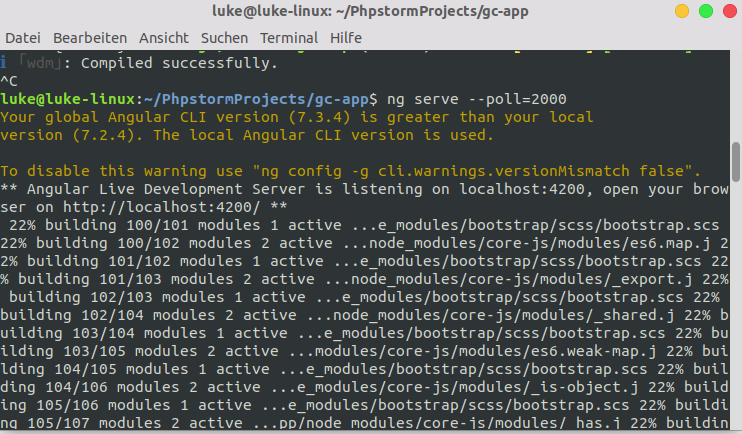
\epsfig{file = grundlagen/images/angularcli.png, width=14.0cm}}
	\caption[Angular CLI Warnung]{\textit{Warnung wegen Versionskonflikt der Angular CLI}}
	\label{fig:ngUpdate}
\end{figure} 
%
Normalerweise kann man diese Meldung ignorieren und sogar ausblenden lassen. Es kann aber unter Umständen sinnvoll sein, wenn etwa eine neue Version neue Features mit sich bringt oder brauchbare Änderungen. Mit dem Befehl \texttt{ng update} ist es innerhalb der Version 7 sehr leicht ein Update vorzunehmen. Nach Ausführen des Befehls sollte die Anwendung mit der aktuellen Version lauffähig sein.
%
%
%%%%%%%%%%%%%%%%%%%%%%%%%%%%%%%%%%%%%%%%%%%%%%%%%%%
%
% A U F B A U 
%
%%%%%%%%%%%%%%%%%%%%%%%%%%%%%%%%%%%%%%%%%%%%%%%%%%%
%
\section{Three.js}
\label{sec:three.js}
%
Schon 2010 begann Ricardo Cabello Miguel die 3D-Bibliothek Three.js zu entwickeln. Mittlerweile ist er unter dem Namen Mr.doob bekannt. Als dann WebGL veröffentlicht wurde, portierte er \textit{Three.js}, um es mit der neuen Technologie zu verwenden. Mr.doob bezeichnete es als \glqq einfach zu implementieren\grqq. Er hatte damals bereits zwei andere Renderer damit gebaut. Seit dieser Zeit hat Three.js an Leistung und Raffinesse zugenommen. Nun ist es zur beliebtesten Wahl für die Erstellung von 3D-Anwendungen mit WebGL geworden. \\
Three.js abstrahiert den Kontext von WebGL und stellt die 3D-Szene als Meshes, Materials und Lightings dar \footnote{Das sind typische Bestandteile einer 3D-Szene die Grafik Programmierer kennen}. Aber Three.js ist mehr als nur eine Abstraktionsschicht für WebGL. Die Three.js-API wurde einfach konzipiert, sodass ein schneller Einstieg möglich ist. Funktionen können ziemlich einfach hinzugefügt und Three.js angepasst werden. Vordefinierte Objekte und Beispiele ermöglichen die Entwicklung von Modellierungsanwendungen bis hin zu Spielen. Auch Animationen sind einfach zu implementieren sowie Interaktionen in der Szene. Neben den Grundfunktionen der Bibliothek gibt es zahlreiche Beispiele und Extras, welche in eigene Projekte eingebunden werden können. Außerdem wurde Three.js so umgesetzt, dass eine hohe Leistung ohne Beeinträchtigung der Usability gewährleistet ist. Zudem gibt es umfangreiche Fehlerprüfungen, Ausnahmen und Konsolenwarnungen, um den Entwickler zu unterstützen.
%
\subsection{Die Szene}
\label{subsec:scene}
%
Die 3D-Bibliothek ist objektorientiert. Das heißt, Programmierer arbeiten mit JavaScript-Objekten, anstatt nur JavaScript-Funktionsaufrufe durchzuführen. Folgendes einfaches Beispiel, zeigt wie eine Szene in Three.js erstellt werden kann. \\
%
\begin{lstlisting}[caption={Erstellung einer Szene in Three.js},label=lst:addscene]
var scene = new THREE.Scene();
\end{lstlisting}
%
Über verschiedene Funktionen können dann die weiteren Bestandteile einer Szene hinzugefügt werden und anschließend mit dem Renderer gerendert werden. Da Angular auf TypeScript basiert, muss man bei der Implementierung einer Szene in Angular ein paar Dinge beachten. Diese werden in Kapitel 4 genauer erläutert. In diesem Teil werden zunächst die wesentlichen Bestandteile der Three.js Szene vorgestellt. Differenzierte Erklärungen zu Three.js sind in der offiziellen Dokumentation zu finden \footnote{http://threejs.org/docs}.
%
\paragraph{Kamera}
Es gibt verschiedene Kameratypen. Normalerweise wird immer die \textit{PerspectiveCamera} verwendet. Deshalb wird in dieser Arbeit nicht weiter auf die anderen Typen eingegangen. Die Kamera wird auch als Objekt in der Szene angelegt. Dabei müssen verschiedene Eigenschaften wie Seitenverhältnis und Position der Kamera angegeben werden.
%
\paragraph{Renderer}
Damit eine Szene gerendert werden kann, wird der Renderer benötigt. Hierbei handelt es sich schlichtweg um einen WebGL-Renderer. Der wird dann in ein \texttt{<canvas>}-Element eingefügt um die Szene darin darzustellen.
%
\paragraph{Lighting}
Damit Objekte der Szene sichtbar werden, muss ein \textit{light} oder sogar mehrere hinzugefügt werden. Sonst ist die Szene einfach nur schwarz. Three.js hat verschiedene Belichtungstypen wie beispielsweise \textit{AmbientLight} oder \textit{PointLight}.
%
\paragraph{Geometry}
Three.js verfügt über leistungsstarke, benutzerfreundliche Objekte für die 3D-Mathematik, z. B. Matrizen, Projektionen und Vektoren. Man kann auch verschiedene Geometrien erzeugen wie zum Beispiel Würfel, Zylinder oder Kugeln. Im nächsten Kapitel werden wir uns noch anschauen wie man einen Zylinder erstellen kann.
%
\paragraph{Materials}
Materials in Three.js definieren das Aussehen von Objekten. Auch hier gibt es wieder verschiedene Materials, je nach Anwendungsfall\footnote{Aus der 3D-Modellierung sind hier Begriffe wie Lambert oder Phong bekannt. Darauf bauen auch die verschiedenen Materials in der Bibliothek aus.}. Dabei hat man unzählige Möglichkeiten das Aussehen umzusetzten. Man kann auch Texturen auf das Objekt \glqq mappen \grqq. Auch ein aus der 3D-Modellierung bekanntes \textit{UV-Mapping} ist möglich.
%
\paragraph{Mesh}
Ein Mesh fast ein oder mehrere Objekte und Materials und so weiter zusammen. Am Ende wird das Mesh zur Szene hinzugefügt.
%
\subsection{Modelle}
\label{subsec:objekte}
%
Mit Three.js lassen sich ebenfalls Modelle aus 3D Programmen wie Maya oder Cinema4D darstellen. Dazu werden Loader, also Werkzeuge mit denen man Modelle laden kann, verwendet. Sie sind nicht Teil vom Kern des Framework. Sie können nach Bedarf in die Anwendung mit eingebunden werden. Teilweise sind die Loader noch nicht ganz ausgereift oder es gibt manchmal Importierungsprobleme. Einige bekannte Loader sind: \textit{ColladaLoader}\footnote{http://www.khronos.org/collada/}, \textit{OBJLoader}\footnote{http://www.martinreddy.net/gfx/3d/OBJ.spec} und \textit{JSONLoader}. Ein noch recht neuer Loader, der immer wieder auftaucht ist der \textit{glFT-Loader}\footnote{https://github.com/KhronosGroup/glTF/tree/master/specification/2.0} der von den Machen von WebGL entwickelt wurde und laut den Entwicklern noch einfacher und performanter arbeiten soll.
%
\subsection{Events}
\label{subsec:events}
%
Three.js liefert einige Funktionen, die bestimmte Events regeln bzw. festlegen, was zu tun ist, wenn bestimmt Aktionen erfolgen. Zum Beispiel hat das \texttt{<canvas>}-Element eine feste Größe. Wenn das Fenster des Browsers sich verändert, sollte das Element sich jedoch anpassen. Das ist ganz einfach mit einem \textit{EventListner} und der Funktion \texttt{resize} umsetzbar.
Hierbei ergänzen sich \textit{Three.js} und \textit{Angular} sehr gut. In dem Framework wird das ganz einfach mit einem Dekorator realisiert. Mit \texttt{@HostListener} können Ereignisse in Angular gebunden werden. Sogar benutzerdefinierte Ereignisse können erstellt werden.
%
%
%%%%%%%%%%%%%%%%%%%%%%%%%%%%%%%%%%%%%%%%%%%%%%%%%%%
%
% A U F B A U 
%
%%%%%%%%%%%%%%%%%%%%%%%%%%%%%%%%%%%%%%%%%%%%%%%%%%%
%
\section{Responsive Webdesign}
\label{sec:responsive}
%
Der erste Eindruck ist wichtig. Ein Besucher benötigt nur 50 Millisekunden, um sich eine Meinung über eine Website zu bilden. Wenn also die Gestaltung der Webseite keinen guten ersten Eindruck hinterlässt, werden viele potenzielle Kunden einfach gehen\cite{webalive}. Laut einer Umfrage von \textit{clutch.co} sollen in 2019 nahezu alle Webseiten kleinerer Unternehmen mobil freundlich sein. Es ist offensichtlich, dass immer mehr mobile Geräte verwendet werden. Deshalb liegt es auch auf der Hand Webseiten für diese Geräteklasse anzupassen.
Laut einer Studie bevorzugen etwa 3/4 der Benutzer mobil freundliche Webseiten und würden sie auch wieder besuchen \cite{searchenginewatch}.\\
In seinem Artikel Responsive Web Design definiert Ethan Marcotte den Begriff mit 3 Säulen:
\textit{\glqq Fluid grids, flexible images, and media queries\grqq } \cite{marcotte_responsive_2010}.
Er betont aber auch, dass es ein anderes Denken erfordert. \textit{\glqq It’s a mechanical concept, the brainchild of a single person, based on finite, specific elements.\grqq} \cite{gardner_what_2014} Es gibt also keine klare Definition von Responsive Webdesign. Oder anders gesagt:
 \textit{\glqq I can tell you how to do Responsive Web Design. How we make things “responsive” is up to us. All of us.\grqq} \cite{gardner_what_2014}. \\
Auch wenn es keine klare Definition von \textit{responsive Webdesign} gibt, so ist klar was damit gemeint ist. Webseiten und Webanwendungen sind responsive, wenn sie für alle Geräteklassen angepasst und optimiert sind. Wie man das genau gestaltet, liegt bei jedem selbst.
%
%
%%%%%%%%%%%%%%%%%%%%%%%%%%%%%%%%%%%%%%%%%%%%%%%%%%%
%
% A U F B A U 
%
%%%%%%%%%%%%%%%%%%%%%%%%%%%%%%%%%%%%%%%%%%%%%%%%%%%
%
\section{Usability}
\label{sec:usability}
%
Die ISO-Norm 9241 beschreibt eine allgemein gültige Definition von Usability:\\

\textit{\glqq Usability bezeichnet das Außmaß, in dem ein Produkt durch bestimmte Benutzer in einem Nutzungskontext genutzt werden kann, um bestimte Ziele effektiv, effizient und mit Zufriedenheit zu erreichen.\grqq} \cite{din-en-iso-9241-210_ergonomie_2010}\\

Hinter dem englische Begriff \textit{Usability} verbirgt sich also ein umfassenderes Konzept, das allgemein unter \textit{Benutzerfreundlichkeit} verstanden wird. Es beschreibt den Umfang, in dem ein System, ein Produkt oder eine Dienstleistung von bestimmten Benutzern verwendet werden kann, um bestimmte Ziele mit Effizienz und Zufriedenheit in einem bestimmten Nutzungskontext zu erreichen. Jedoch dreht sich nicht alles nur um das Produkt. \textit{\glqq Im Mittelpunkt steht aber immer der User mit seinen Wünschen und Bedürfnissen.\grqq} \cite{von_gizycki_usability_2002}\\

\textit{\glqq Software-Anwendungen oder Produkte weisen eine hohe Usability auf, wenn sie von den vorgesehenen Benutzern einfach erlernt und effizient verwendet werden können und diese damit ihre beabsichtigten Ziele und Aufgaben zufriedenstellend ausführen können. Dazu gehören nicht nur ein stimmiges User Interface, sondern auch die passenden Funktionen, um zum Ziel zu gelangen\grqq} \cite{richter_usability_2016}\\

\paragraph{User Centered Design (UCD)}
\textit{\glqq Hinter diesem Begriff verbirgt sich eine Vielzahl von Gestaltungsprozessen, die den späteren Benutzer ins Zentrum der Entwicklung stellen. Mit der Betonung des Designs wird zum Ausdruck gebracht, dass sowohl Interaktions- als auch Gestaltungsaspekte, also etwa die Gestaltung der Dialogabläufe, die Gestaltung der Form physischer Produkte und Bedienelemente, aber auch das grafische Design, wichtige Bestandteile für eine optimale Benutzung darstellen und von Beginn weg berücksichtigt werden müssen..\grqq} \cite{richter_usability_2016}\\

Wir fassen also zusammen, das \textit{Usability} sich immer um den Benutzer dreht und einfach sowie effiziente Bedienung erfordert. Dabei muss die \textit{Benutzerfreundlichkeit} aber immer im Kontext seiner Verwendung beurteilt werden.
%
%
%%%%%%%%%%%%%%%%%%%%%%%%%%%%%%%%%%%%%%%%%%%%%%%%%%%
%
% A U F B A U 
%
%%%%%%%%%%%%%%%%%%%%%%%%%%%%%%%%%%%%%%%%%%%%%%%%%%%
%
\section{Performance}
\label{sec:performance}
%
\textit{Die Leistung vieler Websites hängt von der Auslastung der Website zu Spitzenzeiten unter verschiedenen Bedingungen ab. Leistungstests werden normalerweise in einer vernünftig simulierten Umgebung mit Hilfe von Leistungstestwerkzeugen durchgeführt. Die Leistung einer Website hängt jedoch von verschiedenen Parametern ab, und jeder Parameter muss unter verschiedenen Belastungsniveaus getestet werden.} Aufgrund der Komplexität von Websites ist es nicht möglich, einen gemeinsamen Nenner für Leistungsparameter zum Testen der Website zu zeichnen. Verschiedene Teile der Website müssen mit unterschiedlichen Parametern unter verschiedenen Bedingungen und Belastungsniveaus getestet werden. In solchen Fällen muss die Website in viele Komponenten zerlegt werden, die das Verhalten verschiedener Geschäftskomponenten darstellen. Diese Geschäftskomponenten werden verschiedenen Objekten zugeordnet, die das Verhalten und die Struktur des Teils der Website wirklich darstellen. Diese Objekte werden Leistungstests mit verschiedenen Parametern und Belastungsniveaus unterzogen. In diesem Dokument wird der neue Testprozess angesprochen, bei dem das Konzept der Zerlegung des Verhaltens der Website in testbare Komponenten verwendet wird, die auf testbare Objekte abgebildet werden. Diese überprüfbaren Objekte werden Leistungstests unter verschiedenen Leistungsparametern und Belastungsniveaus unterzogen.\\

Mit diesem Kapitel wurden alle relevanten Grundlagen für die Umsetzung des Projekts erläutert. Der Leser sollte nun ein Grundwissen von Angular und WebGL haben und ein Grundverständnis von SPAs und komponentenbasierter Programmierung. Auch wurden die wichtigen Begriffe responsive Webdesign, Performance und Usability definiert.